\documentclass[a4paper,12pt]{article}
\usepackage[margin=0.5in]{geometry}
\usepackage{graphicx}
\usepackage{hyperref}
\usepackage{tocloft}
\usepackage{multicol}

\title{\textbf{\Huge KöMaLtár\\\large Az unalomtár}}
\author{Valamennyi KöMaL feladatra adott megoldásomat összegyüjtő \LaTeX\ dokumentum.}
\date{} % Üres dátum, hogy ne jelenjen meg dátum

\renewcommand{\cftsecleader}{\cftdotfill{\cftdotsep}}
\begin{document}

\maketitle

\section*{Tartalomjegyzék}

Csak kattints az adott feladatszámra, és már rögtön oda is navigáltál!
\\\\ K. jelű feladatok:\\\break
\hyperref[par:1]{K.799.}\ \ \ \
\hyperref[par:2]{K.800.}\ \ \ \
\hyperref[par:3]{K.801.}\ \ \ \
\\\\ K/C. jelű feladatok:\\\break
\hyperref[par:4]{K/C.802.}\ \ \ \
\hyperref[par:5]{K/C.803.}\ \ \ \
\\\\ C. jelű feladatok:\\\break
\hyperref[par:6]{C.1798.}\ \ \ \
\hyperref[par:7]{C.1800.}\ \ \ \
\hyperref[par:8]{C.1801.}\ \ \ \
\\\\ B. jelű feladatok:\\\break
Hamarosan...
\\\\ A. jelű feladatpróbálkozások:\\
Na azért ez már túlzás...

\newpage

\section*{\Large K.799.}\label{par:1}
\subsection*{Feladat}
Misi egy olyan utcában lakik, amelyben csupa családi ház van. Ha az utca elejétől elindulunk, és megszámoljuk, hogy Misiék azon az oldalon hányadik házban laknak, akkor pontosan kétszer akkora eredményt kapunk, mint ha azt számoljuk meg, hogy az utca végétől számítva hányadik házban laknak. Az utcában a házakat az utca elejétől kezdve folyamatosan számozzák 1-től úgy, hogy a páratlan számú házak a bal oldalon, a páros számú házak a jobb oldalon vannak. Misiék az utca elejétől indulva a bal oldalon laknak. Ha az utca végétől kezdve számoznák a házakat, akkor Misiék házszáma 25-tel lenne kisebb, mint amennyi jelenleg. Hány ház van Misiék oldalán az utcában összesen? 
\subsection*{Megoldás}
Lorem Ipsum...

\section*{\Large K.800.}\label{par:2}
\subsection*{Feladat}
Négy különböző pozitív prímszám összege 50. Melyik négy prímszám lehet ez?

\section*{\Large K.801.}\label{par:3}
\subsection*{Feladat}
n, mint egy-egy betűnek. Az edények oldalnézeti képe látható a másik ábrán, egy 10 cm oldalhosszúságú négyzetekből álló rács elé állítva. Az edények felül nyitottak, vastagságuk 10 cm. Mindkettőbe belehelyezünk egy-egy vékony kis gumicsövet, amelyek leérnek az aljukig, és ezeken keresztül vízzel töltjük meg mindkét edényt. Percenként 1 liter víz folyik be a csövön keresztül mindegyik edénybe. Hány perc alatt telik meg az egyik, illetve a másik edény? Ábrázoljuk az egyes edényekben lévő víz magasságának időbeli alakulását grafikonon. (Az edények falának vastagságát hagyjuk figyelmen kívül.) 
\begin{figure}[htp]
\centering
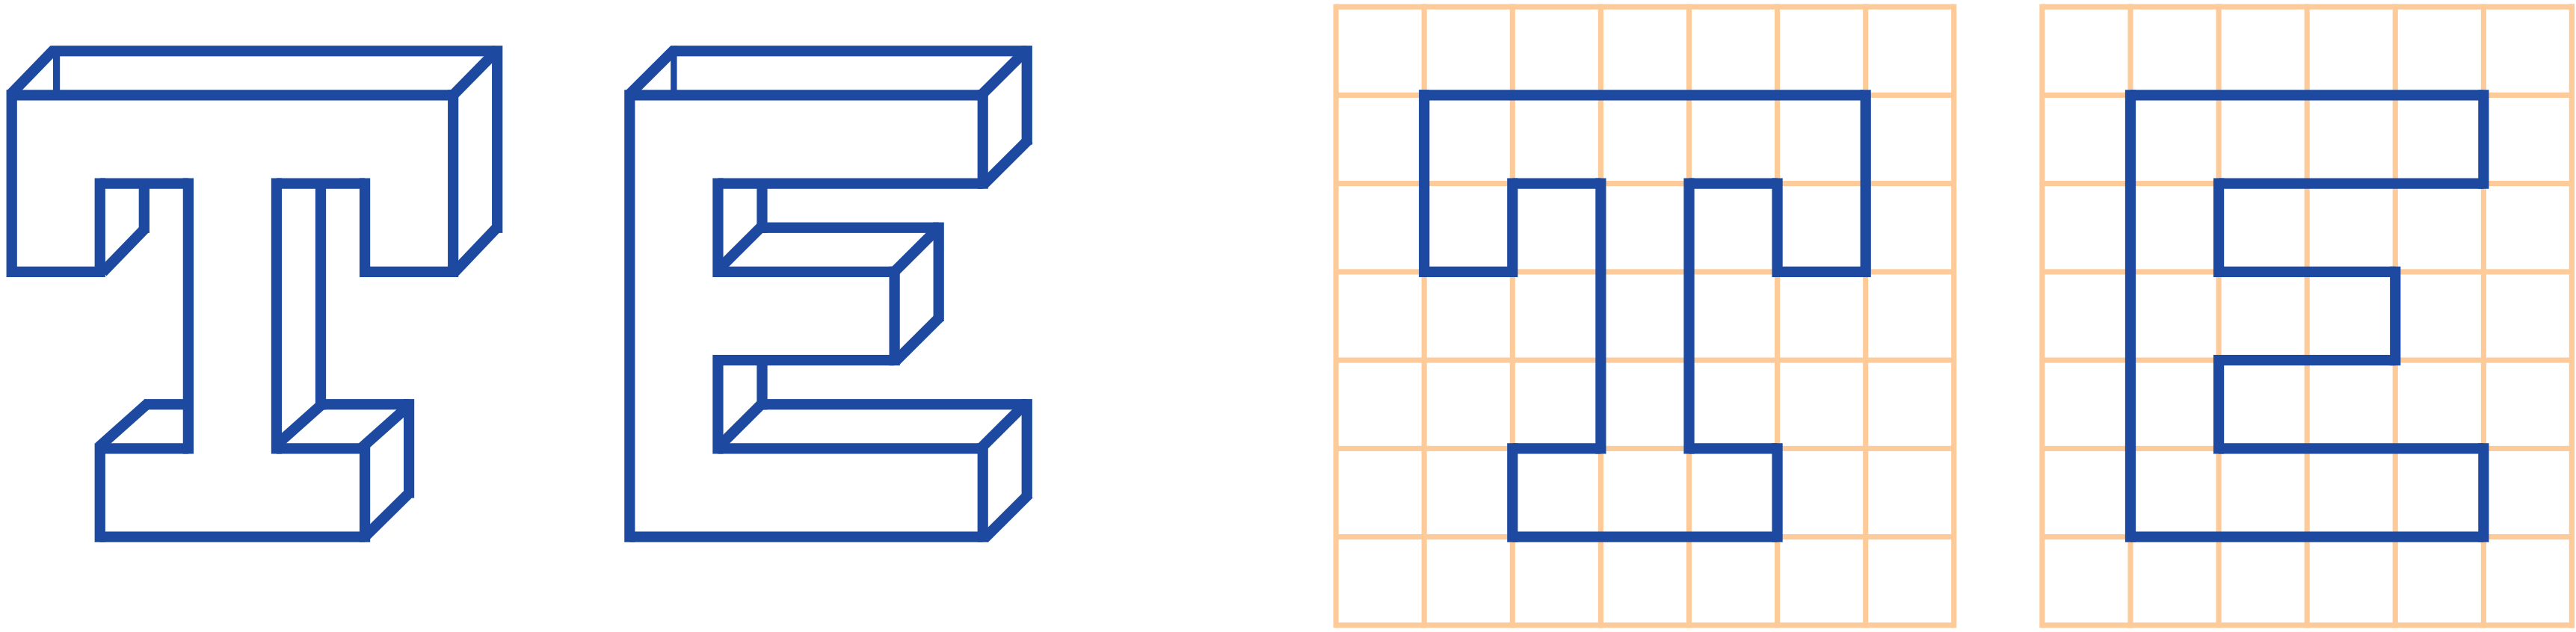
\includegraphics[scale=1.00]{/home/kmark7/FujitsuEgyetem/2023_2024_2felev/KöMaLtár/kepek/k801abra.png}
\label{}
\end{figure}
\subsection*{Megoldás}
Lorem Ipsum...

\section*{\Large K/C.802.}\label{par:4}
\subsection*{Feladat}
Legyen az ABCD négyzet CD oldalának tetszőleges belső pontja Q. Az AQ egyenesre állítsunk merőlegest a B csúcsból, legyen ennek AQ-val vett metszéspontja P. Legyen továbbá a négyzet átlóinak metszéspontja K. Mutassuk meg, hogy a PK egyenes felezi a QPB szöget. 
\begin{figure}[htp]
\centering
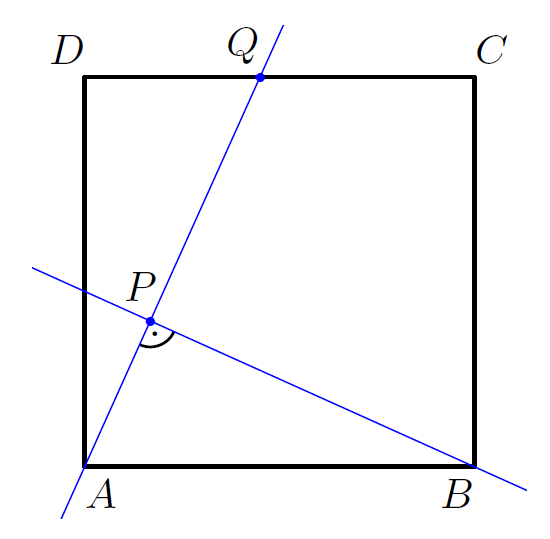
\includegraphics[scale=1.00]{/home/kmark7/FujitsuEgyetem/2023_2024_2felev/KöMaLtár/kepek/kc802abra.png}
\label{}
\end{figure}
\subsection*{Megoldás}
Lorem Ipsum...

\section*{\Large K/C.803.}\label{par:5}
\subsection*{Feladat}
Egy táborban 24 gyerek kivételével mindenki egyke (nincs testvére), 18 gyerek kivételével mindenkinek egy testvére van, 14 gyerek kivételével pedig mindenkinek két testvére van. Hányan lehetnek azok ebben a táborban, akiknek 2-nél több testvérük van, ha tudjuk, hogy van legalább egy egyke, és mindenkinek az összes testvére is ott nyaral a táborban? 
\subsection*{Megoldás}
Lorem Ipsum...

\section*{\Large C.1798.}\label{par:6}
\subsection*{Feladat}
Határozzuk meg a
$$ \left(p+\frac{1}{p}\right)\cdot\left(x-\frac{1}{x}\right)+\left(p-\frac{1}{p}\right)\cdot\left(x+\frac{1}{x}\right)=4px+5+\frac{1}{p} $$
egyenlet összes egész megoldását, ha a p paraméter egész szám. 
\subsection*{Megoldás}
Lorem Ipsum...

\section*{\Large C.1800.}\label{par:7}
\subsection*{Feladat}
Mutassuk meg, hogy ha n természetes szám, akkor a
$$ \Bigl[\sqrt{16n+21}; \sqrt{16n+24}\Bigr] $$
intervallumban nincs egész szám. 
\subsection*{Megoldás}
Lorem Ipsum...

\section*{\Large C.1801.}\label{par:8}
\subsection*{Feladat}
Legyen az $a_n$ sorozat a következő: $a_1=2$ és $a_n=a_{n-1}+2n$. Mennyi a sorozat első 2024 tagjának reciprokösszege? (Vagyis mennyi az $\frac{1}{a_1}+\frac{1}{a_2}+\frac{1}{a_3}+ \dots +\frac{1}{a_{2024}}$ kifejezés értéke?)
\subsection*{Megoldás}
Lorem Ipsum...

\end{document}
